\chapter{Theory and Background} \label{ch:background}
This chapter provides the theoretical foundation for the thesis, focusing strictly on the mechanics of sequential modeling and the time-shift anomaly. Section~\ref{sec:bg:models} introduces the deep learning architectures. Section~\ref{sec:bg:losses} details the mathematical formulations of the evaluated loss functions. Section~\ref{sec:bg:metrics} defines the point-wise and event-centric evaluation metrics.

% ================================================================
\section{Deep Learning for Time Series Forecasting} \label{sec:bg:models}
% ================================================================
\subsection{Long Short-Term Memory Networks} \label{sec:bg:models:lstm}
\begin{planned}
    \item Theoretical foundation of recurrent neural networks for sequential data and the resolution of the vanishing gradient problem.
    \item Mathematical mechanics of the input, forget, and output gating mechanisms.
    \item Brief specification of the chosen baseline recurrent network topology (two stacked layers, hidden size 256), illustrated in Fig.~\ref{fig:bg:lstm_arch}.
\end{planned}

\begin{figure}[H]
    \centering
    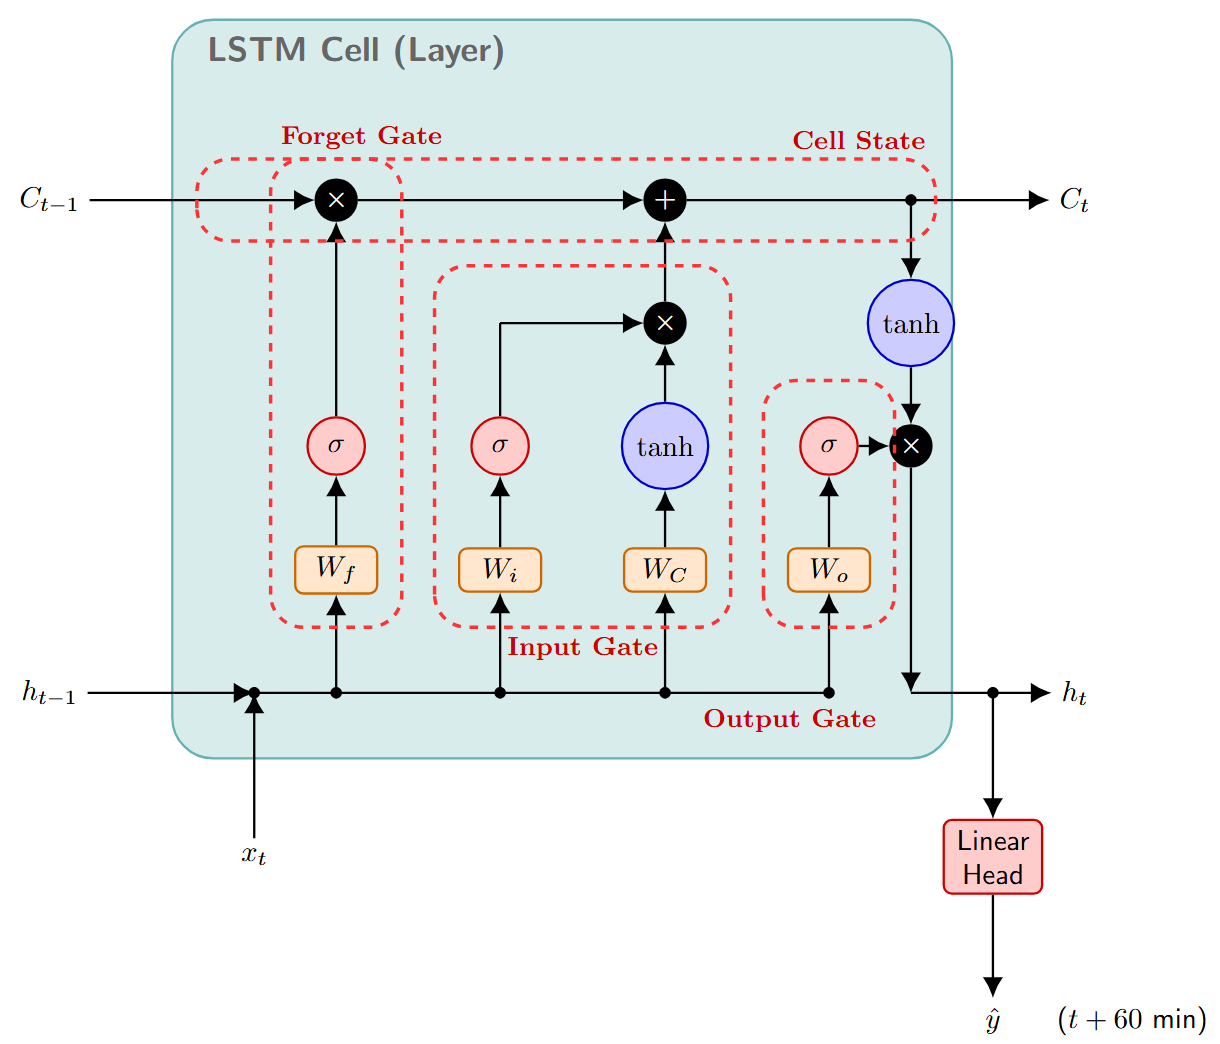
\includegraphics[width=0.65\textwidth]{lstm_cell.png}
    \caption[Architecture of the LSTM model]{Architecture of the LSTM model used as the recurrent baseline. The input is a 24-step lookback window representing 120~minutes of CGM data. Based on \citet{hochreiter1997lstm}.}
    \label{fig:bg:lstm_arch}
\end{figure}

\subsection{PatchTST} \label{sec:bg:models:patchtst}
\begin{planned}
    \item Review of self-attention mechanisms and the core design of the PatchTST architecture (segmentation into overlapping patches), illustrated in Fig.~\ref{fig:bg:patchtst_arch}.
    \item Mathematical framework of Reversible Instance Normalisation (RevIN) utilised to stabilise training.
    \item Analysis of the structural consequence of instance normalisation, which strips absolute level info and compromises classification against static boundaries.
\end{planned}

\begin{figure}[H]
    \centering
    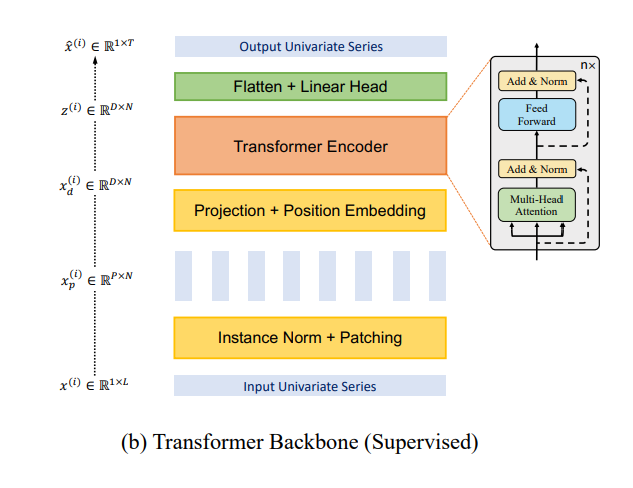
\includegraphics[width=0.65\textwidth]{patchtst_arch_b.png}
    \caption[Architecture of the PatchTST model]{Architecture of the PatchTST model adapted to the CGM setting, incorporating Reversible Instance Normalisation (RevIN). Source: \citet{nie2023patchtst}.}
    \label{fig:bg:patchtst_arch}
\end{figure}

% ================================================================
\section{Loss Functions for Sequential Regression} \label{sec:bg:losses}
% ================================================================

\subsection{Mean Squared Error} \label{sec:bg:losses:mse}
\begin{planned}
    \item Definition of MSE as the average squared difference between each predicted and true value.
    \item Key limitation: MSE penalises a prediction that is correct in shape but slightly shifted in time just as harshly as a completely wrong prediction.
\end{planned}

\begin{figure}[H]
    \centering
    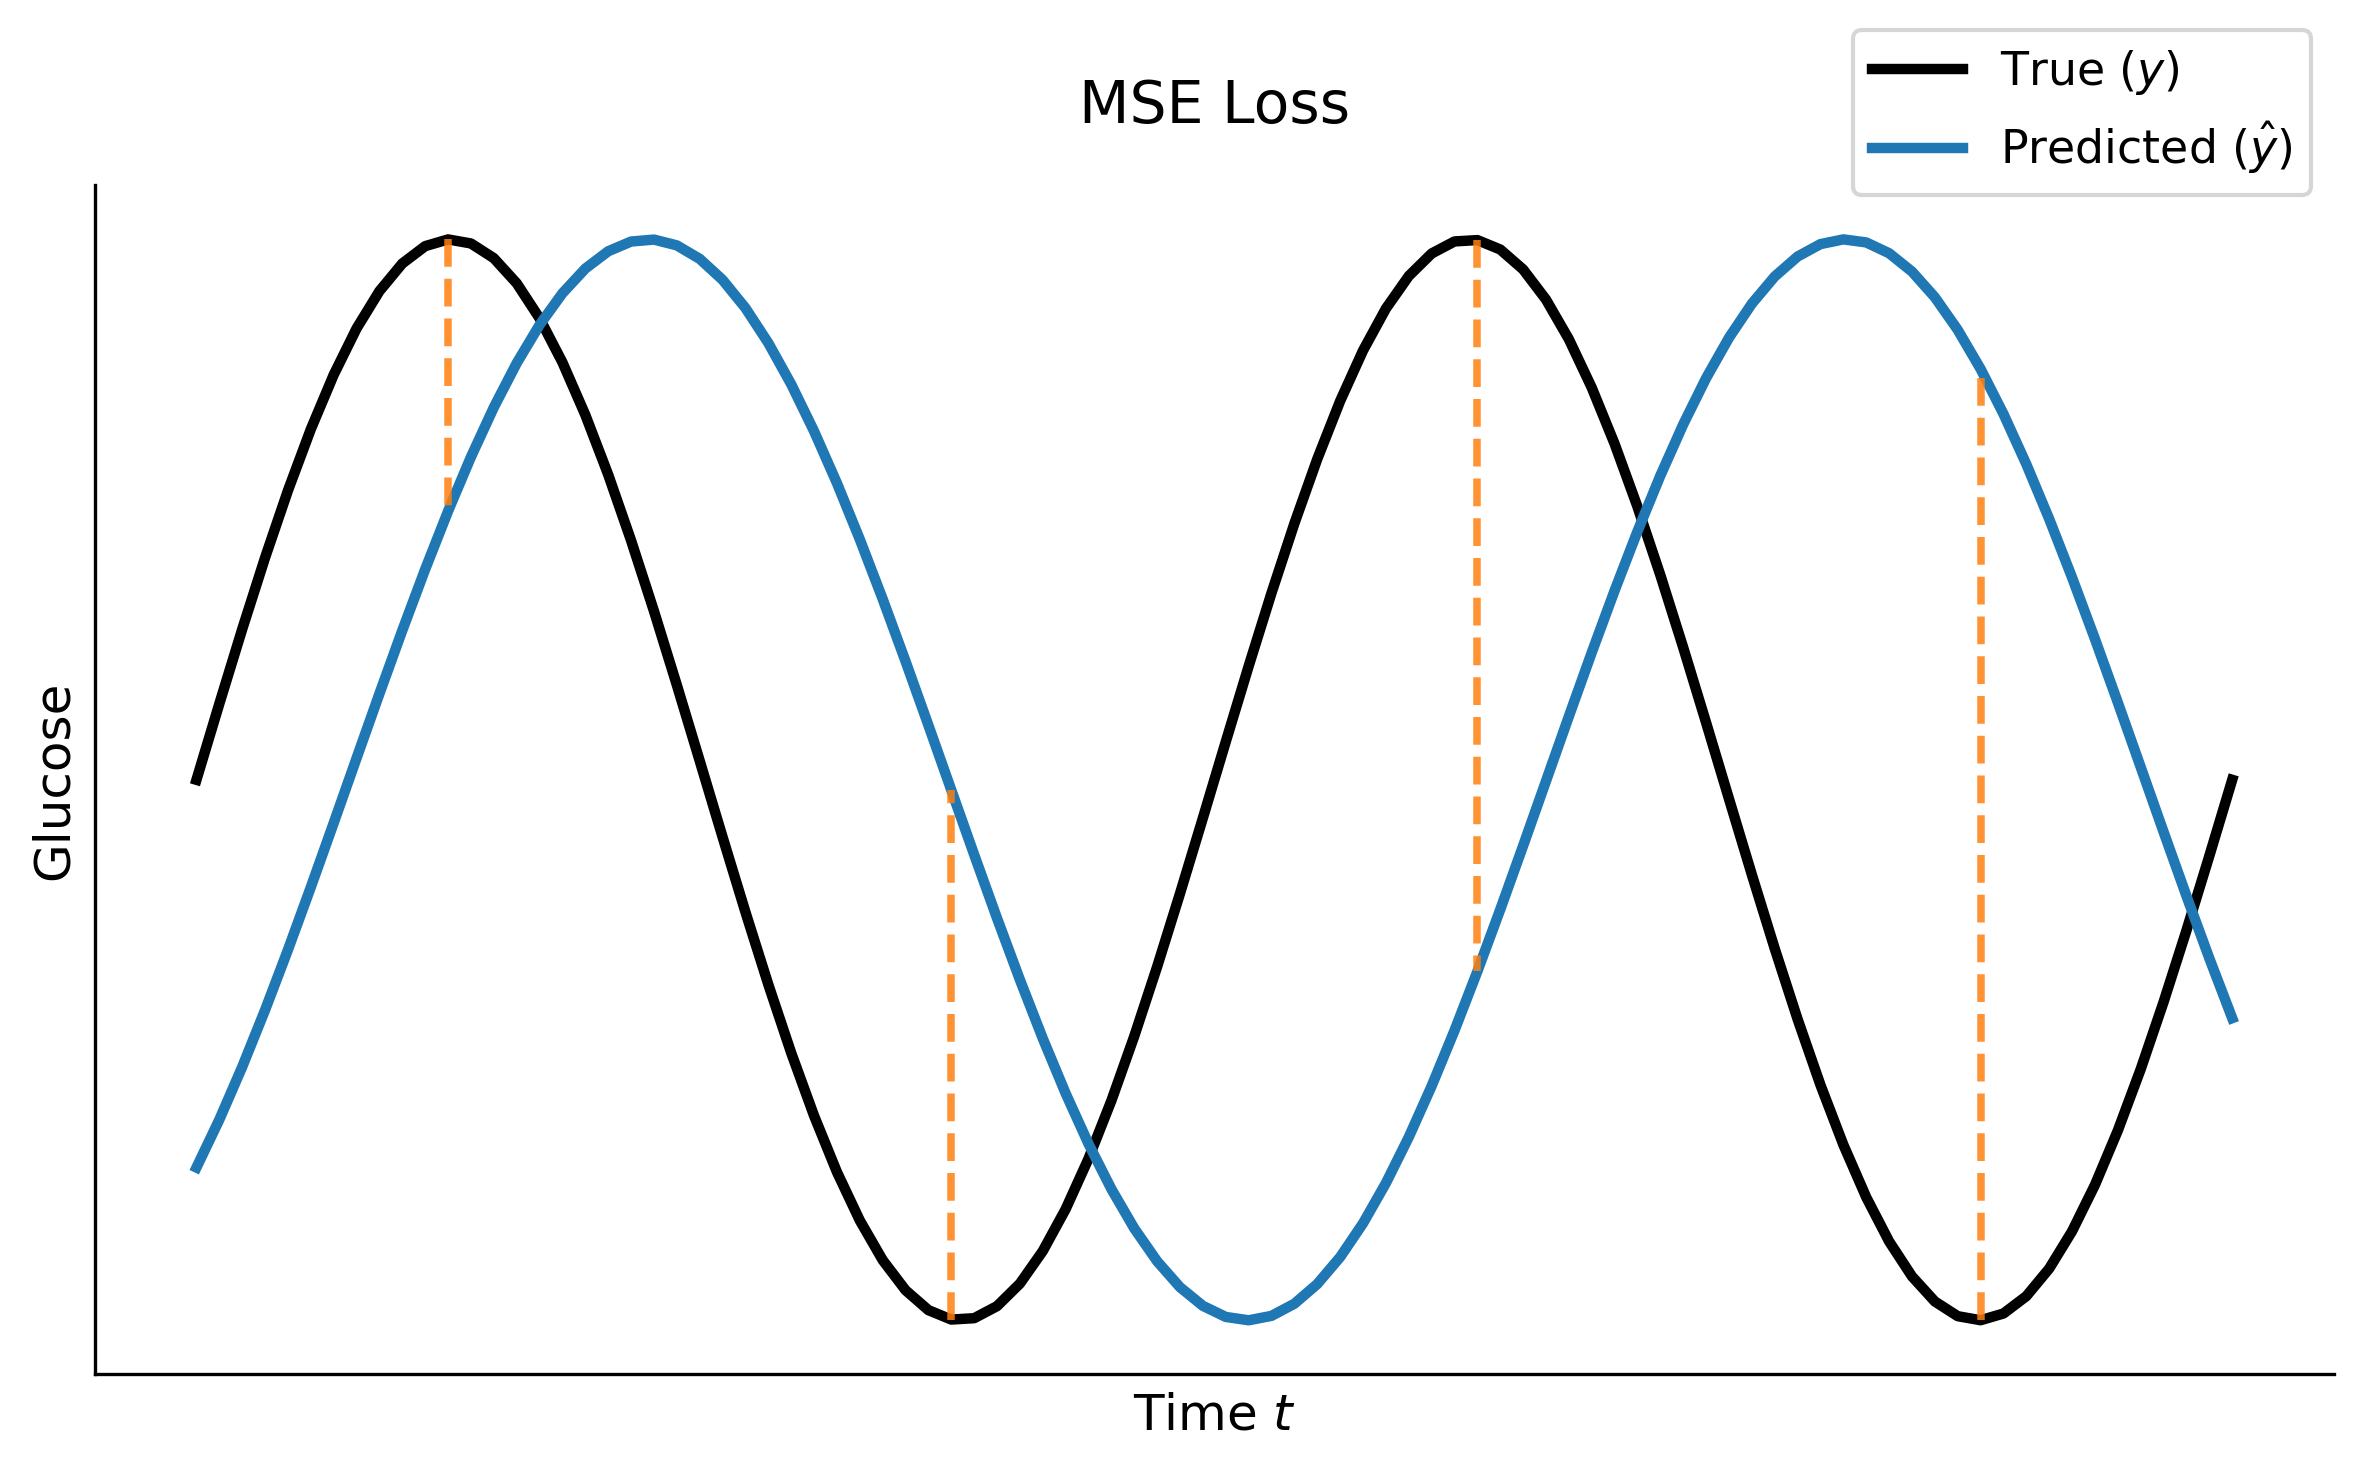
\includegraphics[width=0.75\textwidth]{loss_mse.png}
    \caption{Visual representation of the Mean Squared Error (MSE). The loss is computed as the squared vertical distance between each predicted value and the corresponding true value at the same time step.}
    \label{fig:loss_mse}
\end{figure}

\subsection{Bounded Lag Loss} \label{sec:bg:losses:bl}
\begin{planned}
    \item Description of the Bounded Lag loss, which accepts a prediction as correct if it falls within a fixed time window of the true value, removing the penalty for small timing offsets.
\end{planned}

\begin{figure}[H]
    \centering
    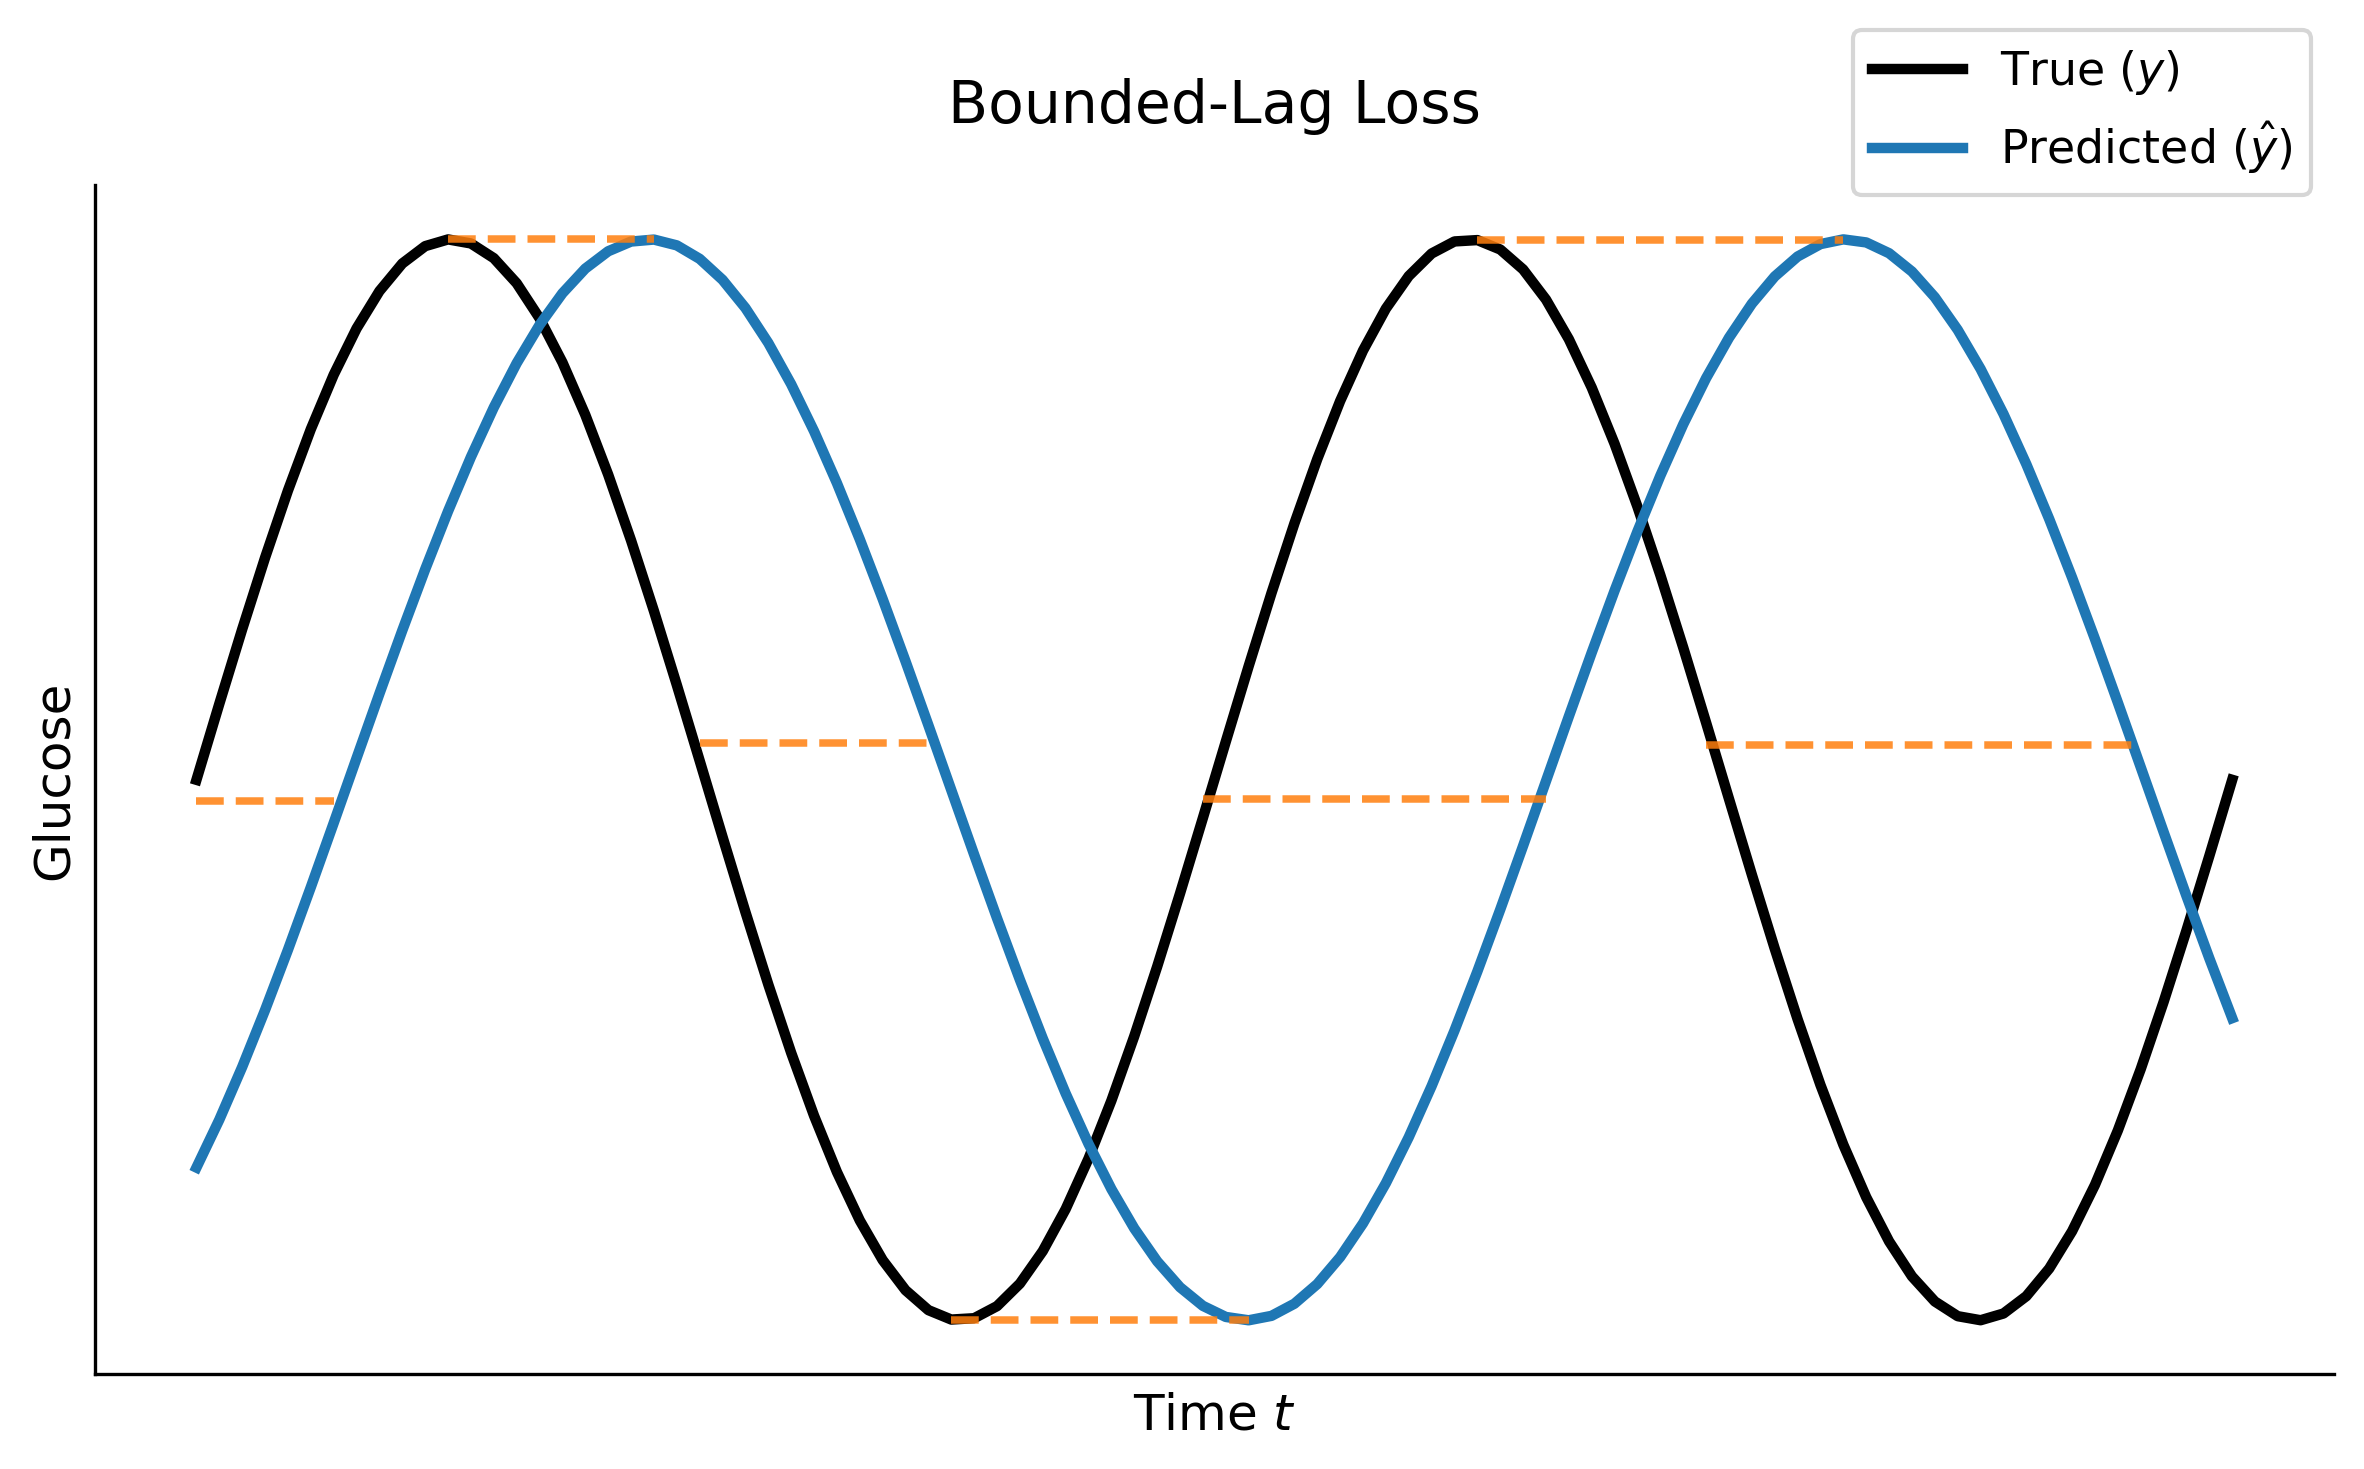
\includegraphics[width=0.75\textwidth]{loss_bounded_lag.png}
    \caption{Visual representation of the Bounded Lag Loss. Temporal shifts within a predefined local neighborhood are tolerated without penalty.}
    \label{fig:loss_bl}
\end{figure}

\subsection{Soft DTW: Differentiable Dynamic Time Warping} \label{sec:bg:losses:sdtw}
\begin{planned}
    \item Description of Soft DTW, which aligns two sequences by warping the time axis to match their shapes, allowing one-to-many correspondences between time steps.
    \item Trade-off: focusing on shape matching reduces the penalty for timing errors but can increase overall amplitude error.
\end{planned}

\begin{figure}[H]
    \centering
    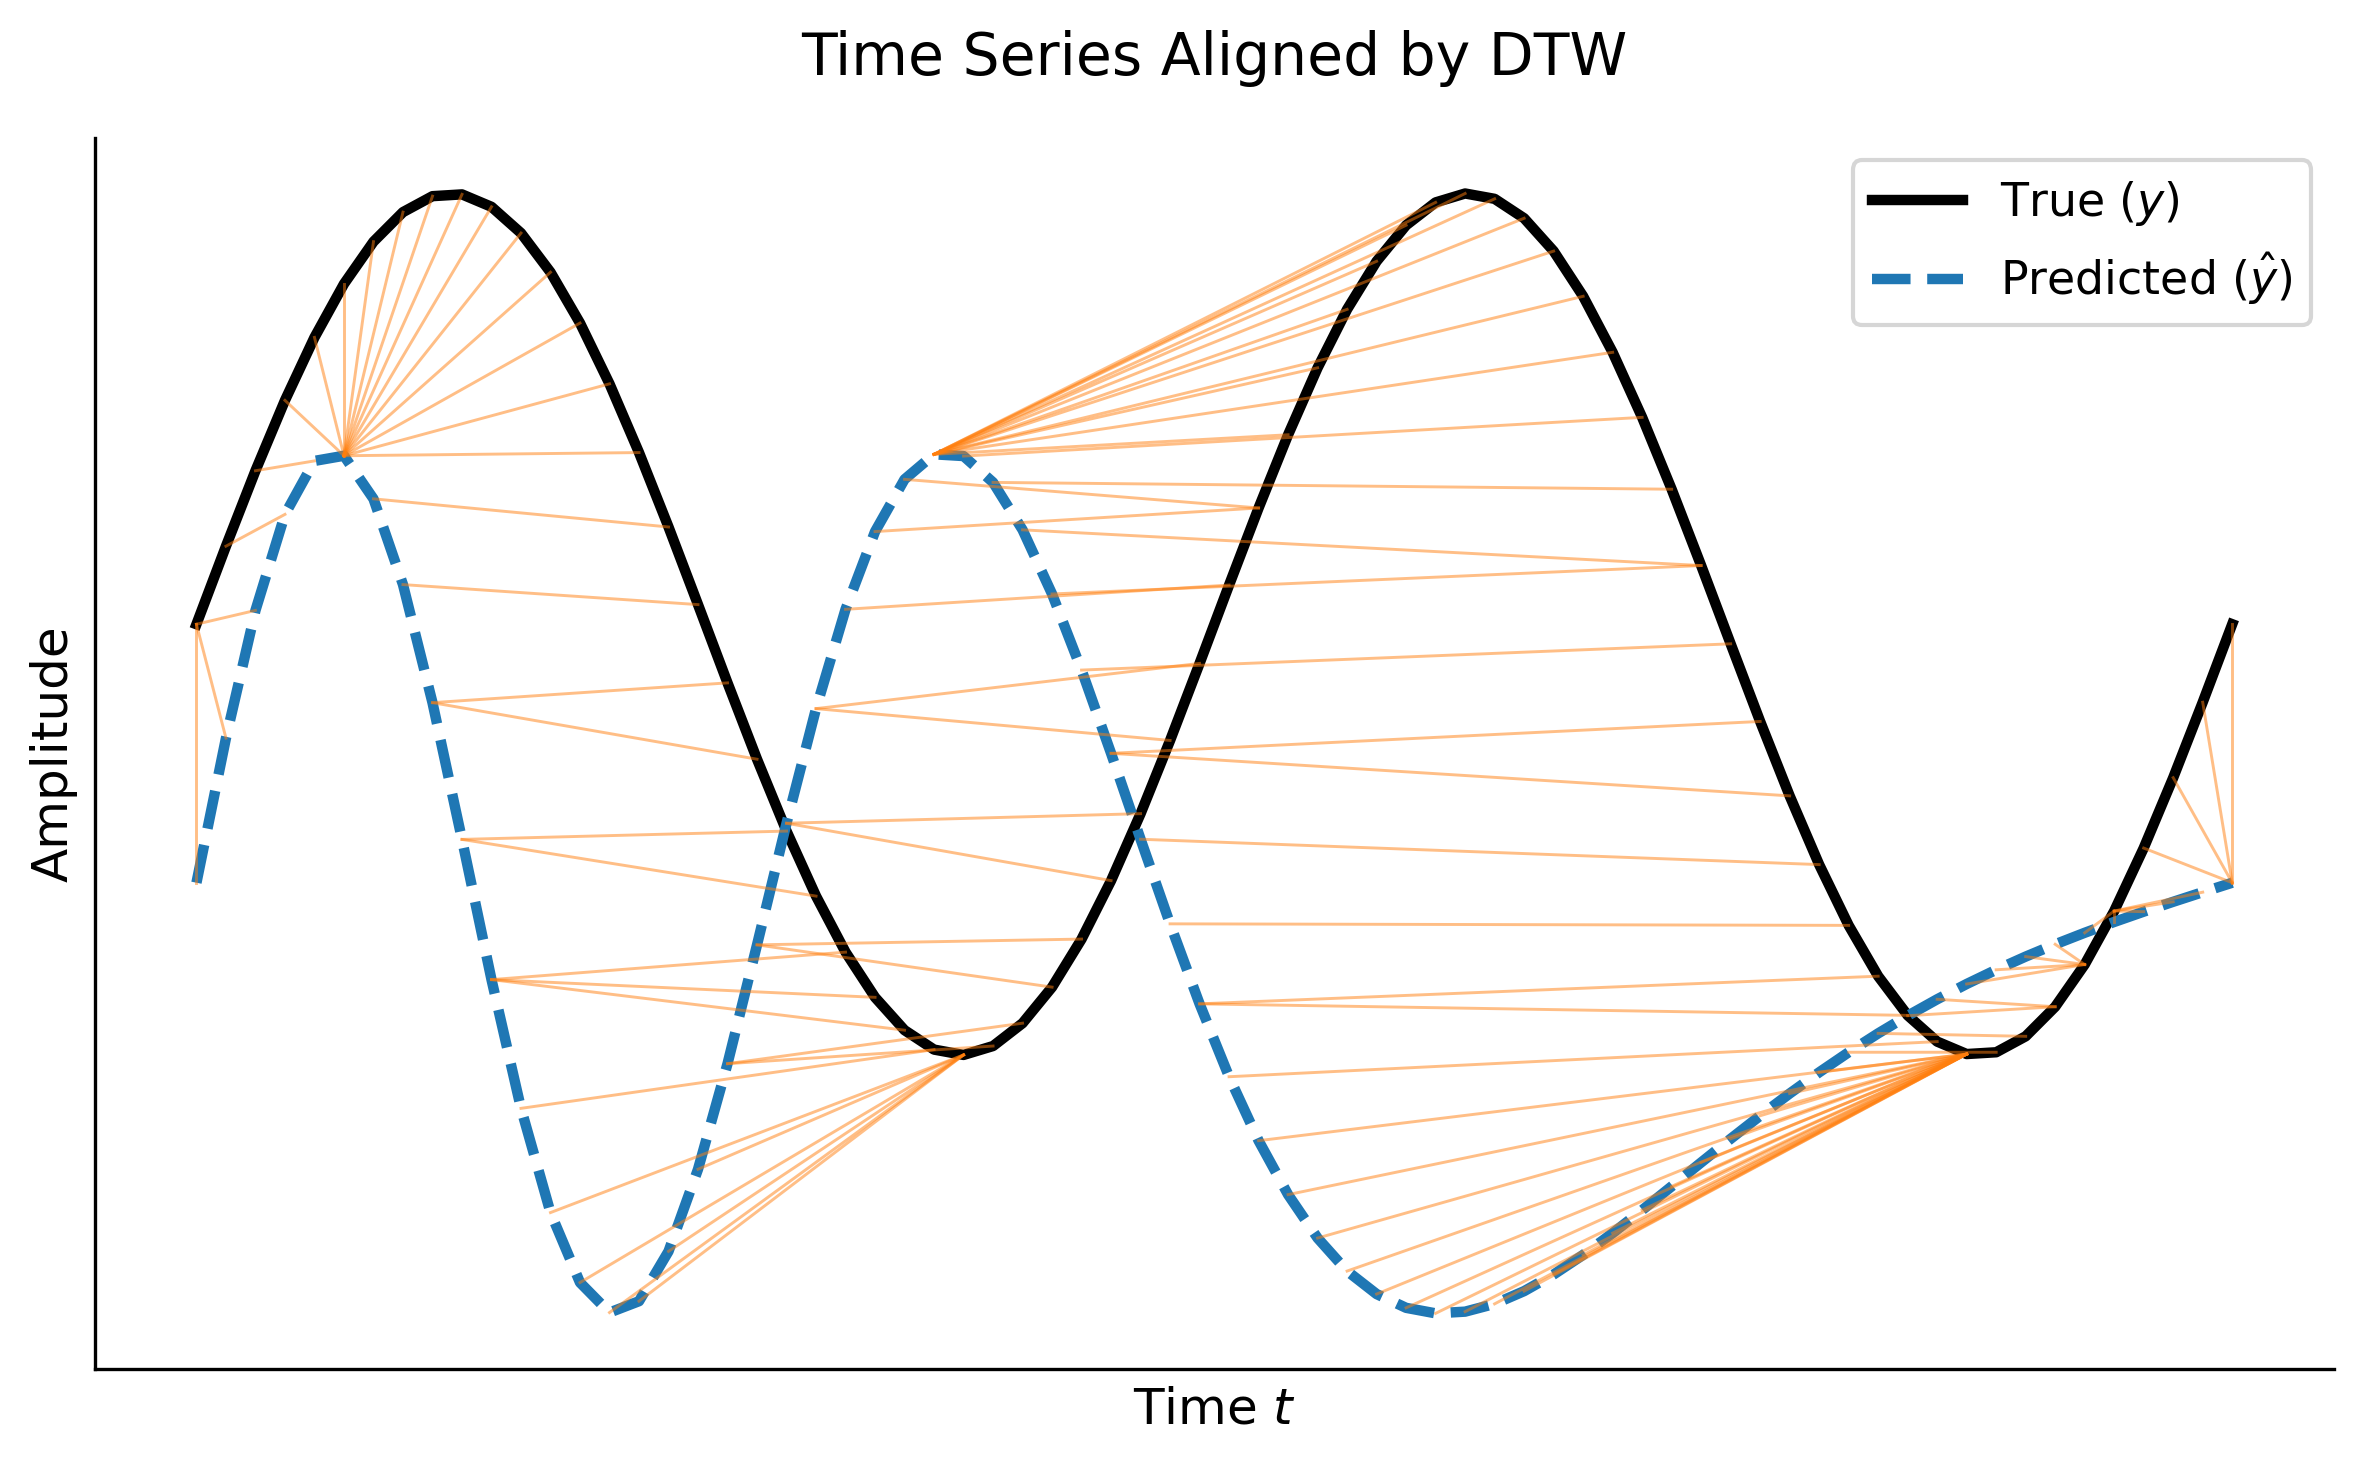
\includegraphics[width=0.75\textwidth]{loss_dtw_alignment.png}
    \caption{Visual representation of the Soft DTW Loss. The algorithm dynamically warps the time axis to match structural shapes using one-to-many alignments.}
    \label{fig:loss_dtw}
\end{figure}

% ================================================================
\section{Evaluation Metrics} \label{sec:bg:metrics}
% ================================================================
\begin{planned}
    \item Mathematical definitions of RMSE and MAE.
    \item Definition of the \texttt{lag\_rmse} diagnostic metric to quantitatively isolate temporal delay components.
    \item Derivation of precision, recall, and harmonic F1/F2 score metrics adapted to the evaluation of highly skewed event detection tasks.
\end{planned}

\begin{figure}[H]
    \centering
    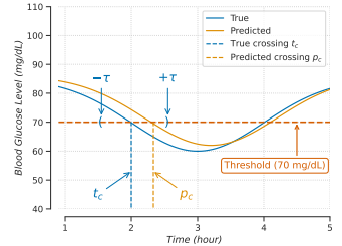
\includegraphics[width=0.7\textwidth]{tau_tolerance.png}
    \caption{Illustration of the event-detection tolerance window $\tau$. The true threshold crossing $t_c$ and the predicted crossing $p_c$ are considered a matched detection if $|t_c - p_c| \leq \tau$. The shaded $\pm\tau$ band around $t_c$ defines the acceptance region; predictions falling outside this window are counted as false positives or misses.}
    \label{fig:bg:tau_tolerance}
\end{figure}


